\section{Integral doble}

\subsection{Qué es una integral doble}

La integral doble permite sumar los valores de una función de dos variables sobre una región del plano. Si $f(x,y)\geq 0$, puede interpretarse como el volumen del sólido que está debajo de la superficie $z=f(x,y)$ y encima de la región $R$ del plano $xy$. Si la función toma valores negativos, la integral representa un volumen con signo: las partes situadas debajo del plano $xy$ restan.

Para empezar, considerese una región rectangular
\[
R=[a,b]\times[c,d]=\{(x,y):a\leq x\leq b,\ c\leq y\leq d\}.
\]
Se divide $R$ en rectángulos pequeños de área $\Delta A$ y, en cada uno, se toma un punto $(x_{ij}^*,y_{ij}^*)$. La suma
\[
\sum_{i,j} f(x_{ij}^*,y_{ij}^*)\,\Delta A
\]
aproxima el volumen. Al hacer los rectángulos cada vez más pequeños, la aproximación se vuelve exacta. Este límite se llama integral doble de $f$ sobre $R$ y se escribe
\[
\iint_R f(x,y)\,dA.
\]

\begin{mydefinition}{Integral doble}
Si existe el límite de las sumas de Riemann anteriores cuando el tamaño de los subrectángulos tiende a cero, se define
\[
\iint_R f(x,y)\,dA
=\lim_{\max\Delta A\to 0}\sum_{i,j}f(x_{ij}^*,y_{ij}^*)\,\Delta A.
\]
En particular, toda función continua en un rectángulo cerrado $R$ tiene integral doble.
\end{mydefinition}

Además del volumen, las integrales dobles se usan para calcular masa de una lámina, carga eléctrica distribuida, valor promedio de una función y otras cantidades repartidas sobre una superficie.

\subsection{Cómo se calcula}

En la práctica, una integral doble sobre un rectángulo se calcula realizando dos integrales ordinarias, una después de la otra. Se puede comenzar por $y$ y después integrar respecto de $x$:
\[
\iint_R f(x,y)\,dA
=\int_a^b\left(\int_c^d f(x,y)\,dy\right)dx.
\]
Al calcular la integral interior respecto de $y$, la variable $x$ se considera una constante. También se puede invertir el orden:
\[
\iint_R f(x,y)\,dA
=\int_c^d\left(\int_a^b f(x,y)\,dx\right)dy.
\]

El procedimiento es el siguiente:
\begin{enumerate}
    \item Identificar la región de integración y sus límites.
    \item Elegir el orden de integración, $dy\,dx$ o $dx\,dy$.
    \item Resolver primero la integral interior, tratando la otra variable como constante.
    \item Sustituir el resultado en la integral exterior y resolverla.
\end{enumerate}

\textbf{Ejemplo.} Calcula
\[
\int_0^2\int_1^3 (x+2y)\,dy\,dx.
\]
Primero se integra respecto de $y$:
\[
\int_1^3(x+2y)\,dy
=\left[xy+y^2\right]_1^3
=3x+9-(x+1)=2x+8.
\]
Después se integra el resultado respecto de $x$:
\[
\int_0^2(2x+8)\,dx
=\left[x^2+8x\right]_0^2
=4+16=20.
\]
Por tanto,
\[
\iint_R(x+2y)\,dA=20,
\qquad
R=[0,2]\times[1,3].
\]

\subsection{Teorema de Fubini}

El teorema de Fubini dice que, para las funciones continuas en un rectángulo dado se puede elegir el orden más conveniente.

\begin{mytheorem}{Teorema de Fubini}
Sea $f$ una función continua en el rectángulo $R=[a,b]\times[c,d]$. Entonces
\[
\iint_R f(x,y)\,dA
=\int_a^b\int_c^d f(x,y)\,dy\,dx
=\int_c^d\int_a^b f(x,y)\,dx\,dy.
\]
\end{mytheorem}

La igualdad no significa que se ignoren los diferenciales: el orden de los límites debe coincidir con la variable de la integral interior. Por ejemplo, en
\[
\int_a^b\int_c^d f(x,y)\,dy\,dx,
\]
primero $y$ recorre el intervalo $[c,d]$ y después $x$ recorre $[a,b]$.

Elegir el orden adecuado puede hacer un cálculo mucho más sencillo. En regiones que no son rectángulos, cambiar el orden sigue siendo posible, pero primero es necesario describir de nuevo los límites de la región.

\subsection{Propiedades}

Sean $f$ y $g$ funciones integrables en una región $R$, y sean $\alpha$ y $\beta$ números reales. Las propiedades principales de la integral doble son las siguientes.

\begin{enumerate}
    \item \textbf{Linealidad.}
    \[
    \iint_R\bigl(\alpha f+\beta g\bigr)\,dA
    =\alpha\iint_R f\,dA+\beta\iint_R g\,dA.
    \]

    \item \textbf{Aditividad respecto de la región.} Si $R$ se divide en dos regiones $R_1$ y $R_2$ que solo comparten una frontera, entonces
    \[
    \iint_R f\,dA
    =\iint_{R_1}f\,dA+\iint_{R_2}f\,dA.
    \]

    \item \textbf{Positividad y comparación.} Si $f(x,y)\geq 0$ en $R$, entonces
    \[
    \iint_R f\,dA\geq 0.
    \]
    Si $f(x,y)\leq g(x,y)$ en $R$, entonces
    \[
    \iint_R f\,dA\leq\iint_R g\,dA.
    \]

    \item \textbf{Cotas.} Si $m\leq f(x,y)\leq M$ en $R$ y $A(R)$ es el área de $R$, entonces
    \[
    m\,A(R)\leq\iint_R f(x,y)\,dA\leq M\,A(R).
    \]

    \item \textbf{Desigualdad del valor absoluto.}
    \[
    \left|\iint_R f\,dA\right|
    \leq\iint_R|f|\,dA.
    \]

    \item \textbf{Producto de funciones separables.} Si $R=[a,b]\times[c,d]$ y $f(x,y)=p(x)q(y)$, entonces
    \[
    \iint_R p(x)q(y)\,dA
    =\left(\int_a^b p(x)\,dx\right)
     \left(\int_c^d q(y)\,dy\right).
    \]
\end{enumerate}

Estas propiedades son las mismas ideas conocidas de las integrales de una variable, ahora aplicadas a una región del plano.

\subsection{Integrales dobles en regiones generales}

Hasta ahora se integró sobre rectángulos. Sin embargo, muchas regiones importantes están delimitadas por rectas, parábolas, circunferencias u otras curvas. Una región general es una región $R$ del plano que puede describirse mediante límites que dependen de una de las variables.

La idea no cambia: la integral doble suma los valores de $f$ sobre toda la región. Lo que cambia es que los extremos de la integral interior ya no son necesariamente constantes. Para plantear correctamente una integral, conviene seguir estos pasos:
\begin{enumerate}
    \item Dibujar la región $R$ en el plano $xy$.
    \item Elegir rebanadas verticales u horizontales.
    \item Leer los límites de cada rebanada en el dibujo.
    \item Escribir la integral iterada y calcularla.
\end{enumerate}

\shorthandoff{>}

\subsection{Regiones orientadas verticalmente (Tipo I)}

Una región es de \textbf{Tipo I} cuando una recta vertical corta a la región en un solo segmento. Se describe como
\[
R=\{(x,y):a\leq x\leq b,\ g_1(x)\leq y\leq g_2(x)\}.
\]
Para cada valor fijo de $x$, $y$ comienza en la curva inferior $g_1(x)$ y termina en la curva superior $g_2(x)$. 
\[
\iint_R f(x,y)\,dA
=\int_a^b\int_{g_1(x)}^{g_2(x)}f(x,y)\,dy\,dx.
\]

\begin{center}
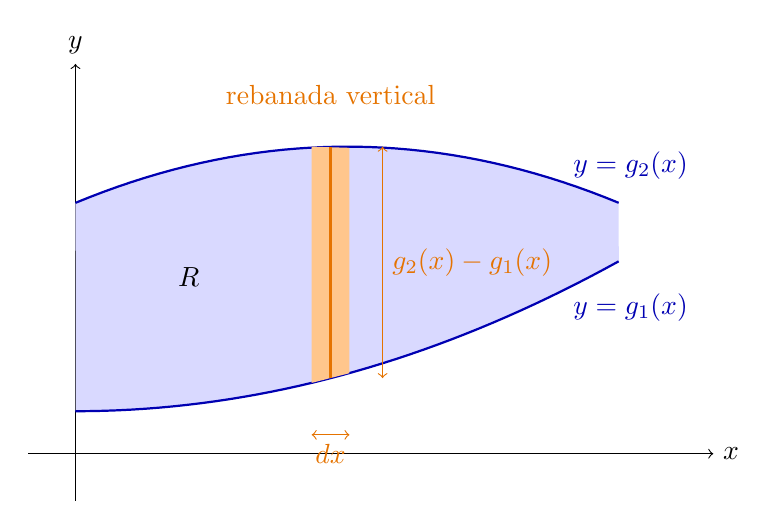
\begin{tikzpicture}[scale=3]
    \draw[->] (-0.2,0) -- (2.7,0) node[right] {$x$};
    \draw[->] (0,-0.2) -- (0,1.65) node[above] {$y$};
    \fill[blue!15] plot[domain=0:2.3, samples=40] (\x,{1.3-0.18*(\x-1.15)*(\x-1.15)}) --
        plot[domain=2.3:0, samples=40] (\x,{0.18+0.12*\x*\x}) -- cycle;
    \draw[blue!70!black, thick] plot[domain=0:2.3, samples=40] (\x,{1.3-0.18*(\x-1.15)*(\x-1.15)});
    \draw[blue!70!black, thick] plot[domain=0:2.3, samples=40] (\x,{0.18+0.12*\x*\x});
    \fill[orange!45] (1,0.3) -- (1.16,0.341) -- (1.16,1.295) -- (1,1.3) -- cycle;
    \draw[orange!90!black, thick] (1.08,0.32) -- (1.08,1.3);
    \draw[<->, orange!90!black] (1.3,0.32) -- (1.3,1.3) node[midway, right] {$g_2(x)-g_1(x)$};
    \draw[<->, orange!90!black] (1,0.08) -- (1.16,0.08) node[midway, below] {$dx$};
    \node[blue!70!black, above] at (2.35,1.12) {$y=g_2(x)$};
    \node[blue!70!black, below] at (2.35,0.72) {$y=g_1(x)$};
    \node at (0.48,0.75) {$R$};
    \node[orange!90!black] at (1.08,1.52) {rebanada vertical};
\end{tikzpicture}
\end{center}

La franja naranja tiene ancho $dx$ y se extiende desde $g_1(x)$ hasta $g_2(x)$; por eso la integral interior se calcula respecto de $y$.

\subsubsection*{Ejemplo 1: región entre una recta y una parábola}

Calcule el volumen bajo $z=x+y$ y sobre la región limitada por $y=x^2$ y $y=x$, para $0\leq x\leq 1$.

\begin{center}
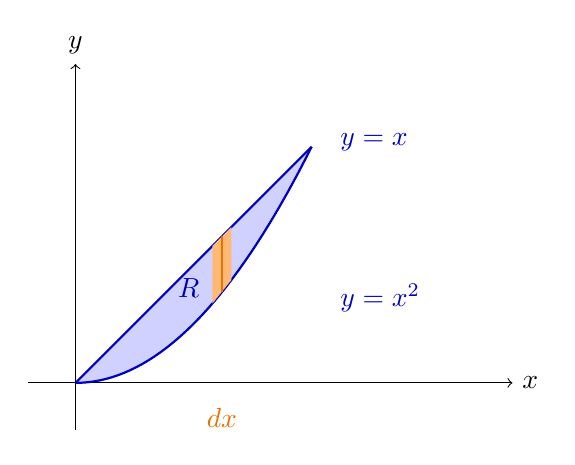
\begin{tikzpicture}[scale=3]
    \draw[->] (-0.2,0) -- (1.85,0) node[right] {$x$};
    \draw[->] (0,-0.2) -- (0,1.35) node[above] {$y$};
    \fill[blue!18] plot[domain=0:1, samples=40] (\x,{\x}) --
        plot[domain=1:0, samples=40] (\x,{\x*\x}) -- cycle;
    \draw[blue!75!black, thick] plot[domain=0:1, samples=40] (\x,{\x});
    \draw[blue!75!black, thick] plot[domain=0:1, samples=40] (\x,{\x*\x});
    \fill[orange!55] (0.58,{0.58*0.58}) -- (0.66,{0.66*0.66}) -- (0.66,0.66) -- (0.58,0.58) -- cycle;
    \draw[orange!90!black, thick] (0.62,{0.62*0.62}) -- (0.62,0.62);
    \node[blue!75!black, anchor=west] at (1.08,1.02) {$y=x$};
    \node[blue!75!black, anchor=west] at (1.08,0.36) {$y=x^2$};
    \node[blue!70!black] at (0.48,0.4) {$R$};
    \node[orange!90!black] at (0.62,-0.15) {$dx$};
\end{tikzpicture}
\end{center}

\begin{center}
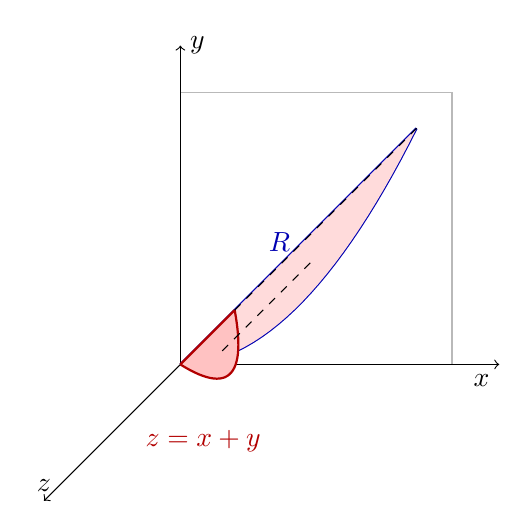
\begin{tikzpicture}[scale=3]
    % El plano xy es la base horizontal del sólido.
    \draw[gray!55] (0,0,0) -- (1.15,0,0) -- (1.15,1.15,0) -- (0,1.15,0) -- cycle;
    \draw[->] (0,0,0) -- (1.35,0,0) node[below left] {$x$};
    \draw[->] (0,0,0) -- (0,1.35,0) node[right] {$y$};
    \draw[->] (0,0,0) -- (0,0,1.5) node[above] {$z$};
    \fill[blue!32] plot[domain=0:1, samples=30] (\x,{\x},0) --
        plot[domain=1:0, samples=30] (\x,{\x*\x},0) -- cycle;
    \draw[blue!70!black, thick] plot[domain=0:1, samples=30] (\x,{\x},0);
    \draw[blue!70!black, thick] plot[domain=0:1, samples=30] (\x,{\x*\x},0);
    \fill[red!14] plot[domain=0:1, samples=30] (\x,{\x*\x},0) --
        plot[domain=1:0, samples=30] (\x,{\x*\x},{\x+\x*\x}) -- cycle;
    \fill[red!24] plot[domain=0:1, samples=30] (\x,{\x},{2*\x}) --
        plot[domain=1:0, samples=30] (\x,{\x*\x},{\x+\x*\x}) -- cycle;
    \draw[red!70!black, thick] plot[domain=0:1, samples=30] (\x,{\x},{2*\x});
    \draw[red!70!black, thick] plot[domain=0:1, samples=30] (\x,{\x*\x},{\x+\x*\x});
    \draw[dashed] (0.55,0.43,0) -- (0.55,0.43,0.98);
    \draw[dashed] (1,1,0) -- (1,1,2);
    \node[blue!70!black] at (0.42,0.52,0) {$R$};
    \node[red!70!black] at (0.72,0.3,1.62) {$z=x+y$};
\end{tikzpicture}
\end{center}

La región es $R=\{(x,y):0\leq x\leq1,\ x^2\leq y\leq x\}$. Por tanto,
\begin{align*}
V&=\int_0^1\int_{x^2}^{x}(x+y)\,dy\,dx\\
 &=\int_0^1\left[xy+\frac{y^2}{2}\right]_{x^2}^{x}dx
 =\int_0^1\left(\frac{3x^2}{2}-x^3-\frac{x^4}{2}\right)dx
 =\frac{3}{20}.
\end{align*}

\subsubsection*{Ejemplo 2: una región triangular}

Calcule el volumen bajo la superficie constante $z=1$ y sobre el triángulo limitado por $x=0$, $y=0$ y $x+y=2$.

\begin{center}
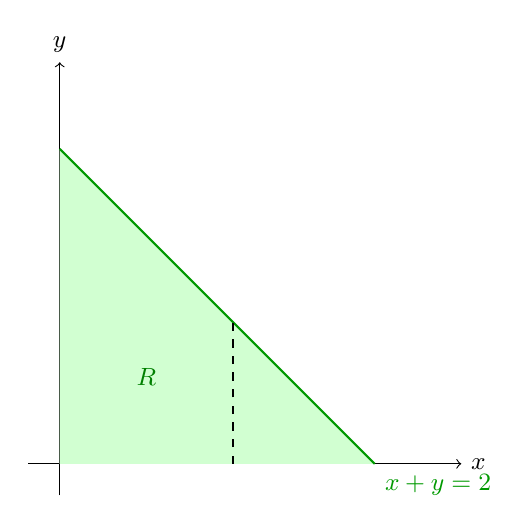
\begin{tikzpicture}[scale=2.0, every node/.style={font=\small}]
    \draw[->] (-0.2,0) -- (2.55,0) node[right] {$x$};
    \draw[->] (0,-0.2) -- (0,2.55) node[above] {$y$};
    \fill[green!18] (0,0) -- (2,0) -- (0,2) -- cycle;
    \draw[green!60!black, thick] (0,2) -- (2,0) node[below right] {$x+y=2$};
    \draw[dashed] (1.1,0) -- (1.1,0.9);
    \node[green!50!black] at (0.55,0.55) {$R$};
\end{tikzpicture}
\end{center}

\begin{center}
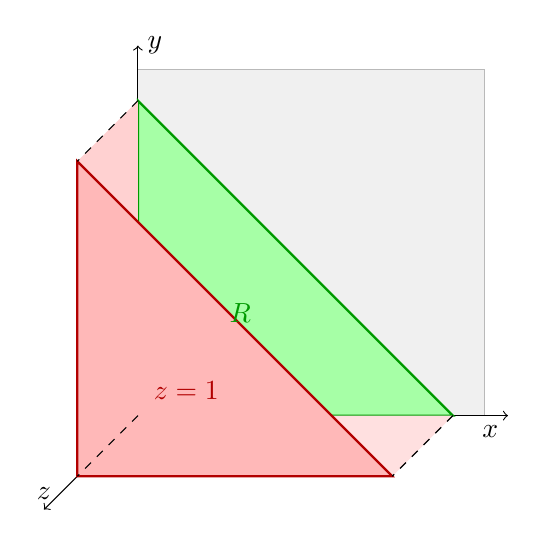
\begin{tikzpicture}[scale=2.0]
    % El plano xy funciona como suelo y z se eleva sobre él.
    \fill[gray!12] (0,0,0) -- (2.2,0,0) -- (2.2,2.2,0) -- (0,2.2,0) -- cycle;
    \draw[gray!55] (0,0,0) -- (2.2,0,0) -- (2.2,2.2,0) -- (0,2.2,0) -- cycle;
    \draw[->] (0,0,0) -- (2.35,0,0) node[below left] {$x$};
    \draw[->] (0,0,0) -- (0,2.35,0) node[right] {$y$};
    \draw[->] (0,0,0) -- (0,0,1.55) node[above] {$z$};
    \fill[green!35] (0,0,0) -- (2,0,0) -- (0,2,0) -- cycle;
    \draw[green!60!black, thick] (0,0,0) -- (2,0,0) -- (0,2,0) -- cycle;
    \fill[red!12] (0,0,0) -- (2,0,0) -- (2,0,1) -- (0,0,1) -- cycle;
    \fill[red!18] (0,0,0) -- (0,2,0) -- (0,2,1) -- (0,0,1) -- cycle;
    \fill[red!28] (0,0,1) -- (2,0,1) -- (0,2,1) -- cycle;
    \draw[red!70!black, thick] (0,0,1) -- (2,0,1) -- (0,2,1) -- cycle;
    \draw[dashed] (0,0,0) -- (0,0,1) (2,0,0) -- (2,0,1) (0,2,0) -- (0,2,1);
    \node[green!60!black] at (0.65,0.65,0) {$R$};
    \node[red!70!black] at (0.75,0.6,1.15) {$z=1$};
\end{tikzpicture}
\end{center}

Una rebanada vertical va desde $y=0$ hasta $y=2-x$, con $0\leq x\leq2$. Así,
\[
V=\int_0^2\int_0^{2-x}1\,dy\,dx
=\int_0^2(2-x)\,dx=2.
\]

\subsubsection*{Ejemplo 3: región entre una curva y una recta}

Calcule el volumen bajo $z=y$ y sobre la región comprendida entre $y=\sin x$ y $y=1$, para $0\leq x\leq\pi$.

\begin{center}
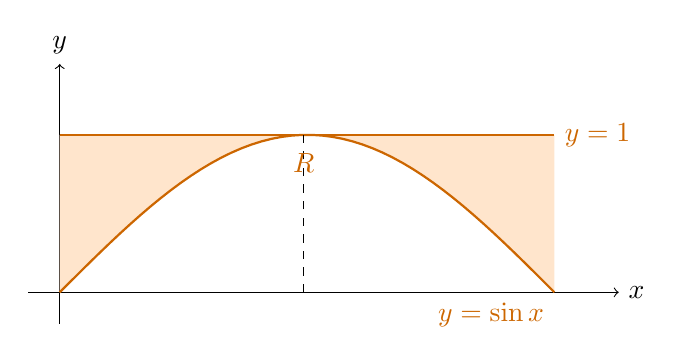
\begin{tikzpicture}[scale=2.0]
    \draw[->] (-0.2,0) -- (3.55,0) node[right] {$x$};
    \draw[->] (0,-0.2) -- (0,1.45) node[above] {$y$};
    \fill[orange!20] plot[domain=0:3.1416, samples=50] (\x,{sin(\x r)}) -- (3.1416,1) -- (0,1) -- cycle;
    \draw[orange!80!black, thick] plot[domain=0:3.1416, samples=50] (\x,{sin(\x r)}) node[below left] {$y=\sin x$};
    \draw[orange!80!black, thick] (0,1) -- (3.1416,1) node[right] {$y=1$};
    \draw[dashed] (1.55,0) -- (1.55,1);
    \node[orange!80!black] at (1.55,0.82) {$R$};
\end{tikzpicture}
\end{center}

\begin{center}
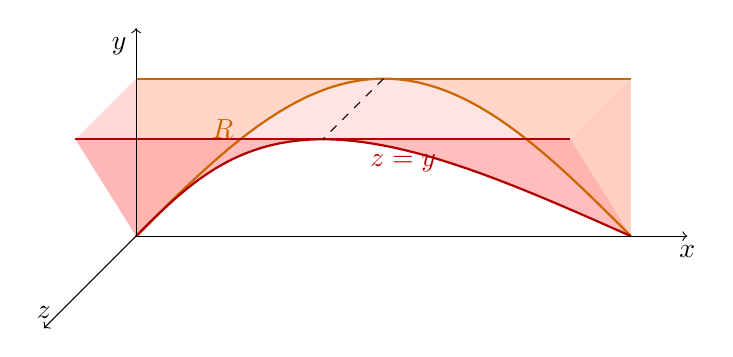
\begin{tikzpicture}[scale=2]
    % La región se reduce a un punto en x=\pi/2; se dibujan sus dos lóbulos por separado.
    \fill[orange!32] plot[domain=0:1.5708, samples=30] (\x,{sin(\x r)},0)
        -- (0,1,0) -- cycle;
    \fill[orange!32] plot[domain=1.5708:3.1416, samples=30] (\x,{sin(\x r)},0)
        -- (3.1416,1,0) -- (1.5708,1,0) -- cycle;

    % Caras laterales del volumen bajo z=y.
    \fill[red!20, opacity=.65] (0,0,0) -- (0,1,0) -- (0,1,1) -- cycle;
    \fill[red!20, opacity=.65] (3.1416,0,0) -- (3.1416,1,0) -- (3.1416,1,1) -- cycle;
    \fill[red!16, opacity=.65] (0,1,0) -- (3.1416,1,0)
        -- (3.1416,1,1) -- (0,1,1) -- cycle;

    % La superficie superior z=y también se divide en los dos lóbulos.
    \fill[red!32, opacity=.80] plot[domain=0:1.5708, samples=30] (\x,{sin(\x r)},{sin(\x r)})
        -- (0,1,1) -- cycle;
    \fill[red!32, opacity=.80] plot[domain=1.5708:3.1416, samples=30] (\x,{sin(\x r)},{sin(\x r)})
        -- (3.1416,1,1) -- (1.5708,1,1) -- cycle;

    \draw[orange!80!black, thick] plot[domain=0:3.1416, samples=50] (\x,{sin(\x r)},0);
    \draw[orange!80!black, thick] (0,1,0) -- (3.1416,1,0);
    \draw[red!70!black, thick] (0,1,1) -- (3.1416,1,1);
    \draw[red!70!black, thick] plot[domain=0:3.1416, samples=50] (\x,{sin(\x r)},{sin(\x r)});
    \draw[dashed] (1.5708,1,0) -- (1.5708,1,1);
    \draw[->] (0,0,0) -- (3.5,0,0) node[below] {$x$};
    \draw[->] (0,0,0) -- (0,1.32,0) node[below left] {$y$};
    \draw[->] (0,0,0) -- (0,0,1.52) node[above] {$z$};
    \node[orange!80!black] at (0.55,0.68,0) {$R$};
    \node[red!70!black] at (2.15,0.92,1.18) {$z=y$};
\end{tikzpicture}
\end{center}

Aquí $\sin x\leq y\leq1$. Entonces
\begin{align*}
V&=\int_0^\pi\int_{\sin x}^{1}y\,dy\,dx
=\frac12\int_0^\pi\bigl(1-\sin^2x\bigr)\,dx
=\frac{\pi}{4}.
\end{align*}

\subsection{Regiones orientadas horizontalmente (Tipo II)}

Una región es de \textbf{Tipo II} cuando una recta horizontal corta a la región en un solo segmento. Se describe como
\[
R=\{(x,y):c\leq y\leq d,\ h_1(y)\leq x\leq h_2(y)\}.
\]
Para cada valor fijo de $y$, $x$ comienza en la curva de la izquierda $h_1(y)$ y termina en la curva de la derecha $h_2(y)$. En este caso,
\[
\iint_R f(x,y)\,dA
=\int_c^d\int_{h_1(y)}^{h_2(y)}f(x,y)\,dx\,dy.
\]

\begin{center}
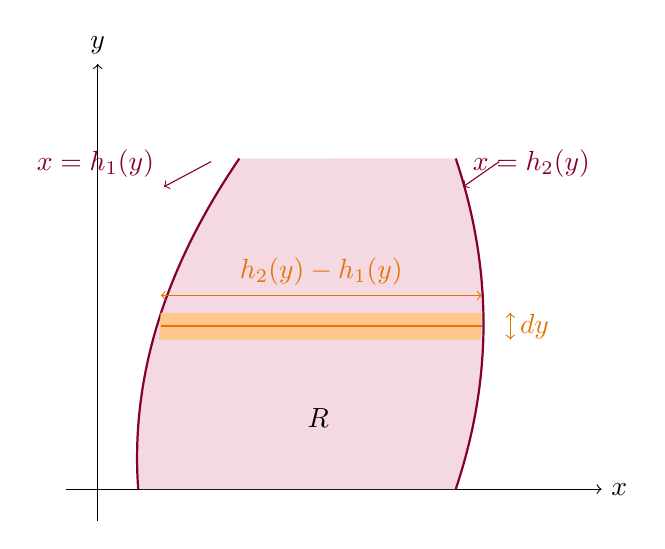
\begin{tikzpicture}[scale=2.0]
    \draw[->] (-0.2,0) -- (3.2,0) node[right] {$x$};
    \draw[->] (0,-0.2) -- (0,2.7) node[above] {$y$};
    \fill[purple!15] plot[domain=0:2.1, samples=40] ({0.25+0.18*(\x-0.2)*(\x-0.2)},\x) --
        plot[domain=2.1:0, samples=40] ({2.45-0.16*(\x-1.05)*(\x-1.05)},\x) -- cycle;
    \draw[purple!70!black, thick] plot[domain=0:2.1, samples=40] ({0.25+0.18*(\x-0.2)*(\x-0.2)},\x);
    \draw[purple!70!black, thick] plot[domain=0:2.1, samples=40] ({2.45-0.16*(\x-1.05)*(\x-1.05)},\x);
    \fill[orange!45] (0.39,0.95) -- (2.43,0.95) -- (2.44,1.12) -- (0.40,1.12) -- cycle;
    \draw[orange!90!black, thick] (0.4,1.035) -- (2.44,1.035);
    \draw[<->, orange!90!black] (0.4,1.23) -- (2.44,1.23) node[midway, above] {$h_2(y)-h_1(y)$};
    \draw[<->, orange!90!black] (2.62,0.95) -- (2.62,1.12) node[midway, right] {$dy$};
    \draw[purple!70!black, ->] (0.72,2.08) -- (0.42,1.92) node[above left] {$x=h_1(y)$};
    \draw[purple!70!black, ->] (2.55,2.08) -- (2.32,1.92) node[above right] {$x=h_2(y)$};
    \node at (1.4,0.45) {$R$};
\end{tikzpicture}
\end{center}

La franja naranja tiene altura $dy$ y se extiende desde $h_1(y)$ hasta $h_2(y)$; por eso la integral interior se calcula respecto de $x$.

\subsubsection*{Ejemplo 1: región entre dos parábolas horizontales}

Calcule el volumen bajo $z=1$ y sobre la región $0\leq y\leq1$ comprendida entre $x=y^2$ y $x=\sqrt{y}$.

\begin{center}
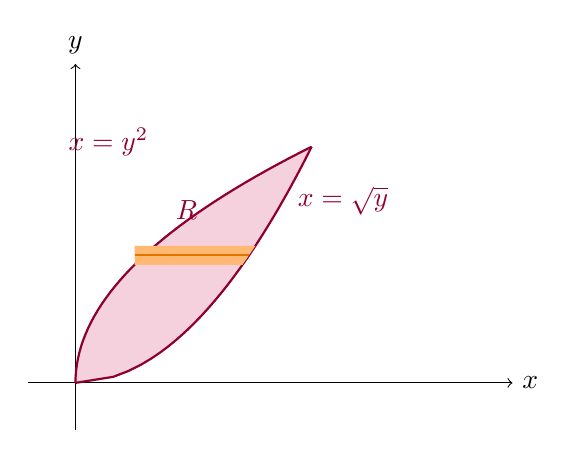
\begin{tikzpicture}[scale=3]
    \draw[->] (-0.2,0) -- (1.85,0) node[right] {$x$};
    \draw[->] (0,-0.2) -- (0,1.35) node[above] {$y$};
    \fill[purple!18] plot[domain=0:1, samples=40] ({\x*\x},\x) --
        plot[domain=1:0, samples=40] ({sqrt(\x)},\x) -- cycle;
    \draw[purple!75!black, thick] plot[domain=0:1, samples=40] ({\x*\x},\x);
    \draw[purple!75!black, thick] plot[domain=0:1, samples=40] ({sqrt(\x)},\x);
    \fill[orange!55] ({0.5*0.5},0.5) -- ({0.5*0.5},0.58) -- ({sqrt(0.58)},0.58) -- ({sqrt(0.5)},0.5) -- cycle;
    \draw[orange!90!black, thick] ({0.5*0.5},0.54) -- ({sqrt(0.54)},0.54);
    \node[purple!75!black, anchor=east] at (0.35,1.02) {$x=y^2$};
    \node[purple!75!black, anchor=west] at (0.9,0.77) {$x=\sqrt y$};
    \node[purple!75!black] at (0.47,0.73) {$R$};
\end{tikzpicture}
\end{center}

\begin{center}
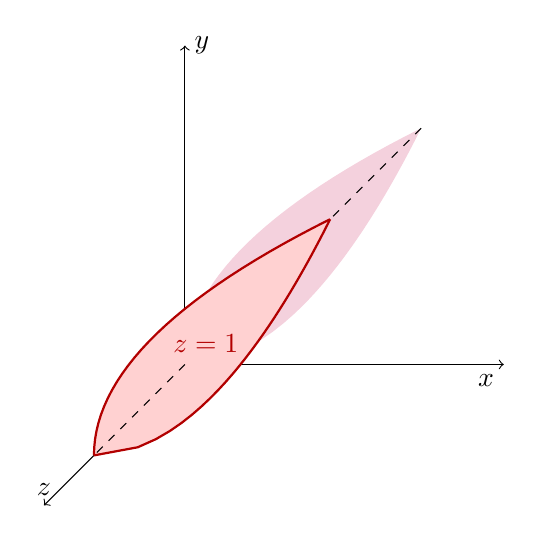
\begin{tikzpicture}[scale=3]
    \draw[->] (0,0,0) -- (1.35,0,0) node[below left] {$x$};
    \draw[->] (0,0,0) -- (0,1.35,0) node[right] {$y$};
    \draw[->] (0,0,0) -- (0,0,1.55) node[above] {$z$};
    \fill[purple!18] plot[domain=0:1, samples=30] ({\x*\x},\x,0) --
        plot[domain=1:0, samples=30] ({sqrt(\x)},\x,0) -- cycle;
    \fill[red!18] plot[domain=0:1, samples=30] ({\x*\x},\x,1) --
        plot[domain=1:0, samples=30] ({sqrt(\x)},\x,1) -- cycle;
    \draw[red!70!black, thick] plot[domain=0:1, samples=30] ({\x*\x},\x,1);
    \draw[red!70!black, thick] plot[domain=0:1, samples=30] ({sqrt(\x)},\x,1);
    \draw[dashed] (0,0,0) -- (0,0,1) (1,1,0) -- (1,1,1);
    \node[red!70!black] at (0.55,0.55,1.2) {$z=1$};
\end{tikzpicture}
\end{center}

Las rebanadas horizontales van de $x=y^2$ a $x=\sqrt y$. Así,
\[
V=\int_0^1\int_{y^2}^{\sqrt y}1\,dx\,dy
=\int_0^1(\sqrt y-y^2)\,dy
=\frac13.
\]

\subsubsection*{Ejemplo 2: un semicírculo}

Calcule el volumen bajo $z=1$ y sobre el semicírculo superior $x^2+y^2\leq4$, $y\geq0$.

\begin{center}
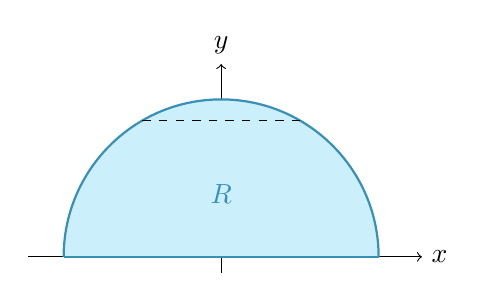
\begin{tikzpicture}[scale=1]
    \draw[->] (-2.45,0) -- (2.55,0) node[right] {$x$};
    \draw[->] (0,-0.2) -- (0,2.45) node[above] {$y$};
    \fill[cyan!20] (-2,0) arc[start angle=180, end angle=0, radius=2] -- cycle;
    \draw[cyan!70!black, thick] (-2,0) arc[start angle=180, end angle=0, radius=2];
    \draw[cyan!70!black, thick] (-2,0) -- (2,0);
    \draw[dashed] (-1,1.732) -- (1,1.732);
    \node[cyan!70!black] at (0,0.8) {$R$};
\end{tikzpicture}
\end{center}

\begin{center}
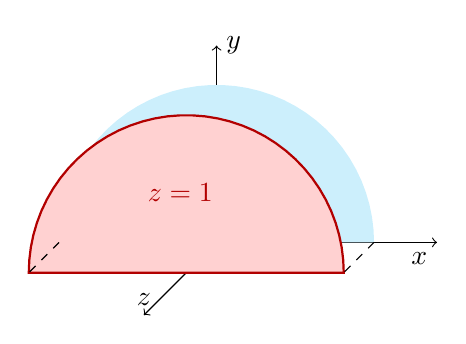
\begin{tikzpicture}[scale=1]
    \draw[->] (-2.35,0,0) -- (2.8,0,0) node[below left] {$x$};
    \draw[->] (0,0,0) -- (0,2.5,0) node[right] {$y$};
    \draw[->] (0,0,0) -- (0,0,2.4) node[above] {$z$};
    \fill[cyan!20] (-2,0,0) plot[domain=180:0, samples=40] ({2*cos(\x)},{2*sin(\x)},0) -- cycle;
    \fill[red!18] (-2,0,1) plot[domain=180:0, samples=40] ({2*cos(\x)},{2*sin(\x)},1) -- cycle;
    \draw[red!70!black, thick] (-2,0,1) plot[domain=180:0, samples=40] ({2*cos(\x)},{2*sin(\x)},1) -- cycle;
    \draw[dashed] (-2,0,0) -- (-2,0,1) (2,0,0) -- (2,0,1);
    \node[red!70!black] at (0,1.1,1.2) {$z=1$};
\end{tikzpicture}
\end{center}

Para cada $y$ entre $0$ y $2$, la rebanada va de $x=-\sqrt{4-y^2}$ a $x=\sqrt{4-y^2}$. Por tanto,
\[
V=\int_0^2\int_{-\sqrt{4-y^2}}^{\sqrt{4-y^2}}1\,dx\,dy
=2\pi.
\]

\subsubsection*{Ejemplo 3: una región triangular con altura variable}

Calcule el volumen bajo $z=x$ y sobre el triángulo limitado por $y=0$, $x=y$ y $x=2-y$, para $0\leq y\leq1$.

\begin{center}
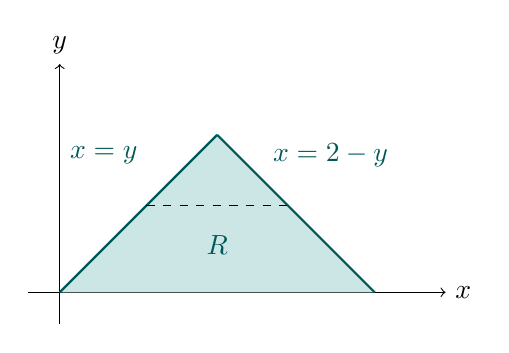
\begin{tikzpicture}[scale=2]
    \draw[->] (-0.2,0) -- (2.45,0) node[right] {$x$};
    \draw[->] (0,-0.2) -- (0,1.45) node[above] {$y$};
    \fill[teal!20] (0,0) -- (2,0) -- (1,1) -- cycle;
    \draw[teal!70!black, thick] (0,0) -- (1,1);
    \draw[teal!70!black, thick] (2,0) -- (1,1);
    \node[teal!70!black] at (0.28,0.87) {$x=y$};
    \node[teal!70!black] at (1.72,0.87) {$x=2-y$};
    \draw[dashed] (0.55,0.55) -- (1.45,0.55);
    \node[teal!70!black] at (1,0.3) {$R$};
\end{tikzpicture}
\end{center}

\begin{center}
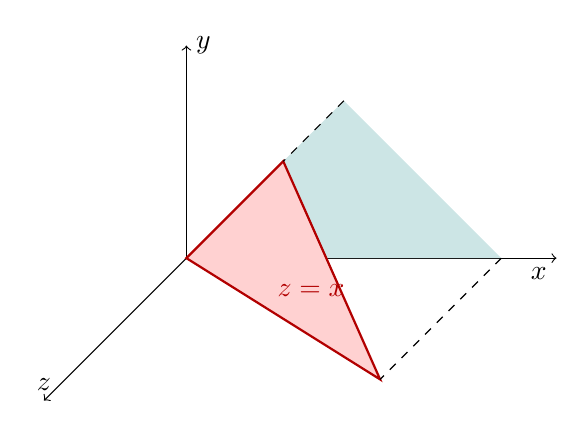
\begin{tikzpicture}[scale=2]
    \draw[->] (0,0,0) -- (2.35,0,0) node[below left] {$x$};
    \draw[->] (0,0,0) -- (0,1.35,0) node[right] {$y$};
    \draw[->] (0,0,0) -- (0,0,2.35) node[above] {$z$};
    \fill[teal!20] (0,0,0) -- (2,0,0) -- (1,1,0) -- cycle;
    \fill[red!18] (0,0,0) -- (2,0,2) -- (1,1,1) -- cycle;
    \draw[red!70!black, thick] (0,0,0) -- (2,0,2) -- (1,1,1) -- cycle;
    \draw[dashed] (2,0,0) -- (2,0,2) (1,1,0) -- (1,1,1);
    \node[red!70!black] at (1.35,0.35,1.45) {$z=x$};
\end{tikzpicture}
\end{center}

Las rebanadas horizontales satisfacen $y\leq x\leq2-y$. Entonces
\begin{align*}
V&=\int_0^1\int_y^{2-y}x\,dx\,dy
=\frac12\int_0^1\bigl[(2-y)^2-y^2\bigr]dy\\
 &=\int_0^1(2-2y)\,dy=1.
\end{align*}

\subsection{Integrales dobles en coordenadas polares}

Las coordenadas polares describen un punto del plano mediante su distancia al origen y el ángulo que forma con el eje $x$. En lugar de usar $(x,y)$, se usa $(r,\theta)$, donde $r\geq0$ y $\theta$ se mide en radianes.

\subsubsection*{¿Por qué se usan?}

Las coordenadas cartesianas son naturales para regiones rectangulares, pero pueden producir límites con raíces cuadradas cuando la frontera es circular. Las coordenadas polares son especialmente útiles cuando:
\begin{itemize}
    \item la región está limitada por círculos, sectores circulares o rayos que salen del origen;
    \item la función depende de $x^2+y^2$, pues $x^2+y^2=r^2$;
    \item la región posee simetría radial.
\end{itemize}
En estos casos, tanto la región como el integrando suelen tomar una forma más simple.

\subsubsection*{El diferencial de área}

Considere el pequeño sector anular comprendido entre los radios $r$ y $r+dr$, y entre los ángulos $\theta$ y $\theta+d\theta$. Sus lados tienen longitudes aproximadas $dr$ y $r\,d\theta$ (arco de circunferencia); por tanto, su área es
\[
dA=r\,dr\,d\theta.
\]

\begin{center}
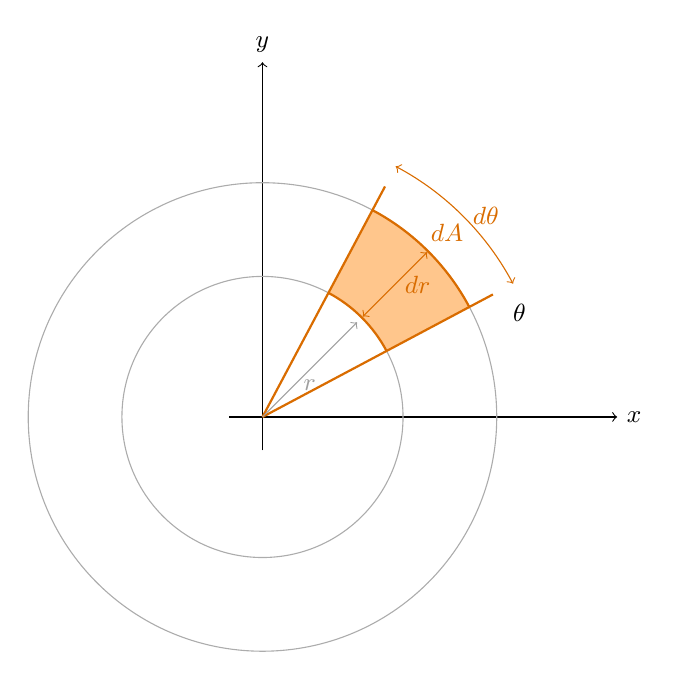
\begin{tikzpicture}[scale=1.7, every node/.style={font=\small}]
    \draw[->] (-0.25,0) -- (2.65,0) node[right] {$x$};
    \draw[->] (0,-0.25) -- (0,2.65) node[above] {$y$};
    \draw[gray!65] (0,0) circle (1.05);
    \draw[gray!65] (0,0) circle (1.75);
    \fill[orange!45] (28:1.05) arc[start angle=28, end angle=62, radius=1.05]
        -- (62:1.75) arc[start angle=62, end angle=28, radius=1.75] -- cycle;
    \draw[orange!85!black, thick] (0,0) -- (28:1.95);
    \draw[orange!85!black, thick] (0,0) -- (62:1.95);
    \draw[orange!85!black, thick] (28:1.05) arc[start angle=28, end angle=62, radius=1.05];
    \draw[orange!85!black, thick] (28:1.75) arc[start angle=28, end angle=62, radius=1.75];
    \draw[<->, orange!85!black] (45:1.06) -- (45:1.74) node[midway, right] {$dr$};
    \draw[<->, orange!85!black] (28:2.12) arc[start angle=28, end angle=62, radius=2.12]
        node[midway, right] {$d\theta$};
    \draw[->, gray!75] (0,0) -- (45:1.0) node[midway, below] {$r$};
    \node[orange!85!black] at (45:1.95) {$dA$};
    \node at (1.92,0.78) {$\theta$};
\end{tikzpicture}
\end{center}

\subsubsection*{Cambio de variable}

La relación entre ambos sistemas es
\[
x=r\cos\theta,\qquad y=r\sin\theta,\qquad x^2+y^2=r^2.
\]
Si la región $R$ se describe en polares por
\[
\alpha\leq\theta\leq\beta,\qquad g_1(\theta)\leq r\leq g_2(\theta),
\]
entonces el cambio de variable para una integral doble es
\[
\iint_R f(x,y)\,dA
=\int_\alpha^\beta\int_{g_1(\theta)}^{g_2(\theta)}
f(r\cos\theta,r\sin\theta)\,r\,dr\,d\theta.
\]
Primero se transforma la región y el integrando; después se añade el factor $r$ del diferencial. El orden de integración también puede intercambiarse si los límites resultan más sencillos.

\subsubsection*{Ejemplo 1: área de un disco}

Calcule el área del disco $x^2+y^2\leq4$.

\begin{center}
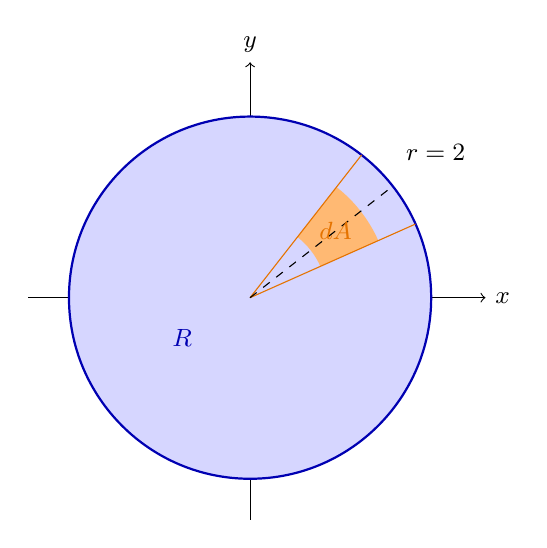
\begin{tikzpicture}[scale=1.15, every node/.style={font=\small}]
    \draw[->] (-2.45,0) -- (2.6,0) node[right] {$x$};
    \draw[->] (0,-2.45) -- (0,2.6) node[above] {$y$};
    \fill[blue!16] (0,0) circle (2);
    \fill[orange!55] (24:0.85) arc[start angle=24, end angle=52, radius=0.85]
        -- (52:1.55) arc[start angle=52, end angle=24, radius=1.55] -- cycle;
    \draw[blue!70!black, thick] (0,0) circle (2);
    \draw[orange!90!black] (0,0) -- (24:2) (0,0) -- (52:2);
    \draw[dashed] (0,0) -- (38:2);
    \node[blue!70!black] at (-0.75,-0.45) {$R$};
    \node[orange!90!black] at (38:1.2) {$dA$};
    \node at (38:2.6) {$r=2$};
\end{tikzpicture}
\end{center}

En coordenadas polares, el disco se describe simplemente por $0\leq r\leq2$ y $0\leq\theta\leq2\pi$. Como el área corresponde a $f(x,y)=1$,
\[
A=\int_0^{2\pi}\int_0^2 r\,dr\,d\theta
=\int_0^{2\pi}\left.\frac{r^2}{2}\right|_0^2d\theta
=4\pi.
\]

\subsubsection*{Ejemplo 2: volumen sobre un semidisco}

Calcule el volumen bajo $z=x^2+y^2$ y sobre el semidisco superior $x^2+y^2\leq4$, $y\geq0$.

\begin{center}
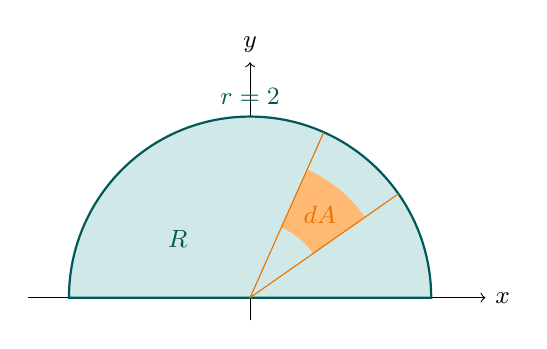
\begin{tikzpicture}[scale=1.15, every node/.style={font=\small}]
    \draw[->] (-2.45,0) -- (2.6,0) node[right] {$x$};
    \draw[->] (0,-0.25) -- (0,2.6) node[above] {$y$};
    \fill[teal!18] (-2,0) arc[start angle=180, end angle=0, radius=2] -- cycle;
    \fill[orange!55] (35:0.85) arc[start angle=35, end angle=66, radius=0.85]
        -- (66:1.55) arc[start angle=66, end angle=35, radius=1.55] -- cycle;
    \draw[teal!70!black, thick] (-2,0) arc[start angle=180, end angle=0, radius=2] -- cycle;
    \draw[orange!90!black] (0,0) -- (35:2) (0,0) -- (66:2);
    \node[teal!70!black] at (-0.8,0.65) {$R$};
    \node[orange!90!black] at (50:1.2) {$dA$};
    \node[teal!70!black] at (0,2.22) {$r=2$};
\end{tikzpicture}
\end{center}

Ahora $x^2+y^2=r^2$, y la región queda dada por $0\leq\theta\leq\pi$, $0\leq r\leq2$. Por ello,
\begin{align*}
V&=\int_0^\pi\int_0^2 r^2\,r\,dr\,d\theta
=\int_0^\pi\left.\frac{r^4}{4}\right|_0^2d\theta\\
&=\int_0^\pi4\,d\theta=4\pi.
\end{align*}

\subsubsection*{Ejemplo 3: un cuarto de corona circular}

Calcule $\iint_R(x+y)\,dA$, donde $R$ es la región del primer cuadrante comprendida entre los círculos $x^2+y^2=1$ y $x^2+y^2=4$.

\begin{center}
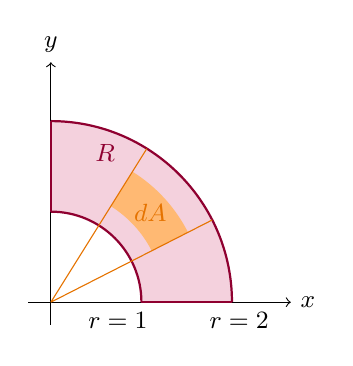
\begin{tikzpicture}[scale=1.15, every node/.style={font=\small}]
    \draw[->] (-0.25,0) -- (2.65,0) node[right] {$x$};
    \draw[->] (0,-0.25) -- (0,2.65) node[above] {$y$};
    \fill[purple!18] (1,0) arc[start angle=0, end angle=90, radius=1]
        -- (90:2) arc[start angle=90, end angle=0, radius=2] -- cycle;
    \fill[orange!55] (27:1.25) arc[start angle=27, end angle=58, radius=1.25]
        -- (58:1.70) arc[start angle=58, end angle=27, radius=1.70] -- cycle;
    \draw[purple!75!black, thick] (1,0) arc[start angle=0, end angle=90, radius=1];
    \draw[purple!75!black, thick] (2,0) arc[start angle=0, end angle=90, radius=2];
    \draw[purple!75!black, thick] (1,0) -- (2,0) (0,1) -- (0,2);
    \draw[orange!90!black] (0,0) -- (27:2) (0,0) -- (58:2);
    \node[purple!75!black] at (70:1.75) {$R$};
    \node[orange!90!black] at (42:1.48) {$dA$};
    \node at (0.74,-0.2) {$r=1$};
    \node at (2.08,-0.2) {$r=2$};
\end{tikzpicture}
\end{center}

La región está delimitada por $0\leq\theta\leq\pi/2$ y $1\leq r\leq2$. Además,
\[
x+y=r\cos\theta+r\sin\theta=r(\cos\theta+\sin\theta).
\]
Así,
\begin{align*}
\iint_R(x+y)\,dA
&=\int_0^{\pi/2}\int_1^2r(\cos\theta+\sin\theta)\,r\,dr\,d\theta\\
&=\left.\frac{r^3}{3}\right|_1^2
\int_0^{\pi/2}(\cos\theta+\sin\theta)\,d\theta\\
&=\frac73\,[\sin\theta-\cos\theta]_0^{\pi/2}
=\frac{14}{3}.
\end{align*}

\subsection{Aplicaciones de la integral doble}

Una integral doble no solo calcula volúmenes. Su idea central es sumar contribuciones muy pequeñas distribuidas sobre una región del plano. Según qué represente la función que se integra, esa suma puede describir la masa de una lámina, su equilibrio o el promedio de una cantidad aleatoria.

\subsubsection*{Masa y densidad superficial}

Una lámina es un objeto plano cuya masa se distribuye sobre una región $R$. La densidad superficial $\rho(x,y)$ indica cuánta masa hay por unidad de área cerca del punto $(x,y)$. Sus unidades son, por ejemplo, $\mathrm{g/cm^2}$ o $\mathrm{kg/m^2}$.

Para un elemento pequeño de área $dA$, la masa es aproximadamente
\[
dm=\rho(x,y)\,dA.
\]
Al sumar todos los elementos de la lámina se obtiene su masa total:
\[
m=\iint_R\rho(x,y)\,dA.
\]
Si $\rho$ es constante, la lámina es homogénea y $m=\rho\,\text{área}(R)$. Cuando $\rho$ varía, las zonas con densidad mayor aportan más masa, aun cuando tengan la misma área que otras zonas.

\begin{center}
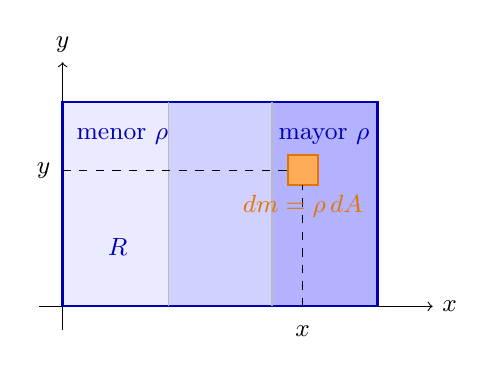
\begin{tikzpicture}[scale=2.0, every node/.style={font=\small}]
    \draw[->] (-0.15,0) -- (2.35,0) node[right] {$x$};
    \draw[->] (0,-0.15) -- (0,1.55) node[above] {$y$};
    \fill[blue!8] (0,0) rectangle (2,1.3);
    \fill[blue!18] (0.67,0) rectangle (1.33,1.3);
    \fill[blue!30] (1.33,0) rectangle (2,1.3);
    \draw[blue!70!black, thick] (0,0) rectangle (2,1.3);
    \draw[gray!55] (0.67,0) -- (0.67,1.3) (1.33,0) -- (1.33,1.3);
    \fill[orange!65] (1.43,0.77) rectangle (1.62,0.96);
    \draw[orange!90!black, thick] (1.43,0.77) rectangle (1.62,0.96);
    \draw[dashed] (1.525,0) -- (1.525,0.77) (0,0.865) -- (1.43,0.865);
    \node[orange!90!black, below] at (1.525,0.77) {$dm=\rho\,dA$};
    \node[blue!70!black] at (0.38,1.08) {menor $\rho$};
    \node[blue!70!black] at (1.66,1.08) {mayor $\rho$};
    \node at (1.525,-0.16) {$x$};
    \node at (-0.12,0.865) {$y$};
    \node[blue!70!black] at (0.35,0.38) {$R$};
\end{tikzpicture}
\end{center}

\subsubsection*{Momentos y centro de masa}

La masa total no dice cómo está repartida la materia. Para medir su tendencia a hacer girar o equilibrar la lámina respecto de un eje se usan los primeros momentos. La distancia de $(x,y)$ al eje $x$ es $y$, y su distancia al eje $y$ es $x$; por eso
\[
M_x=\iint_R y\,\rho(x,y)\,dA,
\qquad
M_y=\iint_R x\,\rho(x,y)\,dA.
\]
El subíndice indica el eje respecto del cual se toma el momento. Por ejemplo, una masa situada muy arriba tiene un brazo de palanca $y$ grande y contribuye mucho a $M_x$.

El centro de masa $(\bar x,\bar y)$ es el punto en que se concentraría toda la masa sin alterar estos primeros momentos. Si $m>0$,
\[
\bar x=\frac{M_y}{m},
\qquad
\bar y=\frac{M_x}{m}.
\]
Así, $\bar x$ se obtiene del momento respecto del eje $y$, pues este eje mide las distancias horizontales. En una lámina homogénea, el centro de masa coincide con el centroide geométrico de la región; con densidad variable se desplaza hacia las zonas más densas.

También existen los segundos momentos o momentos de inercia,
\[
I_x=\iint_R y^2\rho\,dA,
\qquad
I_y=\iint_R x^2\rho\,dA,
\qquad
I_O=\iint_R(x^2+y^2)\rho\,dA.
\]
Estos penalizan cuadráticamente la distancia al eje: describen qué tan difícil es poner la lámina a girar alrededor de un eje.

\subsubsection*{Ejemplo: masa y centro de masa de una lámina no homogénea}

Sea $R=[0,2]\times[0,1]$ y sea $\rho(x,y)=1+x+y$. La densidad aumenta hacia la esquina superior derecha. La masa es
\begin{align*}
m&=\int_0^2\int_0^1(1+x+y)\,dy\,dx
=\int_0^2\left(x+\frac32\right)dx=5.
\end{align*}
Los primeros momentos son
\begin{align*}
M_x&=\int_0^2\int_0^1y(1+x+y)\,dy\,dx=\frac83,\\
M_y&=\int_0^2\int_0^1x(1+x+y)\,dy\,dx=\frac{17}{3}.
\end{align*}
Por tanto,
\[
(\bar x,\bar y)=\left(\frac{M_y}{m},\frac{M_x}{m}\right)
=\left(\frac{17}{15},\frac{8}{15}\right).
\]
El centro de masa está a la derecha y por encima del centro geométrico $(1,1/2)$, tal como anticipa la mayor densidad en esa dirección.

\subsubsection*{Valores esperados de variables aleatorias continuas}

En probabilidad, una función $f_{X,Y}(x,y)$ puede representar la densidad conjunta de dos variables aleatorias continuas $X$ y $Y$. No es una probabilidad puntual: la probabilidad de observar exactamente un solo punto es $0$. La probabilidad aparece al acumular densidad sobre una región $A$:
\[
P\bigl((X,Y)\in A\bigr)=\iint_A f_{X,Y}(x,y)\,dA.
\]
Para que $f_{X,Y}$ sea una densidad válida debe cumplir
\[
f_{X,Y}(x,y)\geq0,
\qquad
\iint_R f_{X,Y}(x,y)\,dA=1.
\]
La segunda condición normaliza toda la masa probabilística a $1$. A diferencia de una densidad de masa, una densidad de probabilidad puede ser mayor que $1$; lo importante es que su integral total sea $1$.

El valor esperado de una cantidad $g(X,Y)$ es su promedio ponderado por la densidad conjunta:
\[
E[g(X,Y)]=\iint_R g(x,y)f_{X,Y}(x,y)\,dA.
\]
En particular,
\[
E[X]=\iint_R x f_{X,Y}(x,y)\,dA,
\qquad
E[Y]=\iint_R y f_{X,Y}(x,y)\,dA.
\]
Haciendo una analogía al centro de masa: la densidad $f_{X,Y}$ ocupa el papel de $\rho$, y $(E[X],E[Y])$ es el centro de masa de una lámina de masa total $1$. El valor esperado no tiene por qué ser el valor más probable ni un valor que se observe en un experimento individual; representa el promedio de muchas repeticiones.

Para estudiar la dispersión y la relación entre las variables se usan
\[
\operatorname{Var}(X)=E[X^2]-E[X]^2,
\qquad
\operatorname{Cov}(X,Y)=E[XY]-E[X]E[Y].
\]
Una covarianza negativa indica que valores grandes de una variable tienden a acompañarse de valores pequeños de la otra. Si $X$ y $Y$ son independientes, entonces $E[XY]=E[X]E[Y]$ y la covarianza es $0$; el recíproco no siempre es cierto.

Las densidades marginales permiten estudiar una variable sin tomar en cuenta la otra:
\[
f_X(x)=\int f_{X,Y}(x,y)\,dy,
\qquad
f_Y(y)=\int f_{X,Y}(x,y)\,dx,
\]
donde cada integral se toma sobre los valores que mantienen a $(x,y)$ dentro de $R$. Estas funciones también se integran a $1$ y permiten calcular, por ejemplo, $E[X]$ con una sola integral.

\subsubsection*{Ejemplo: esperanza y dependencia en una región triangular}

Suponga que la densidad conjunta es uniforme sobre el triángulo
\[
R=\{(x,y):0\leq x\leq1,\ 0\leq y\leq1-x\}.
\]
Como el área del triángulo es $1/2$, la densidad constante que normaliza la probabilidad es $f_{X,Y}(x,y)=2$ sobre $R$ y $0$ fuera de ella.

\begin{center}
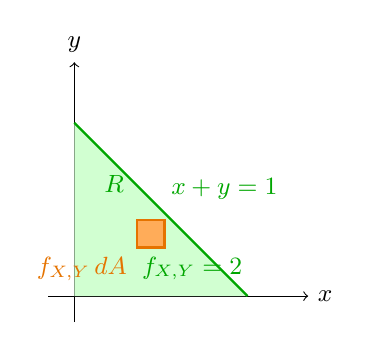
\begin{tikzpicture}[scale=2.2, every node/.style={font=\small}]
    \draw[->] (-0.15,0) -- (1.35,0) node[right] {$x$};
    \draw[->] (0,-0.15) -- (0,1.35) node[above] {$y$};
    \fill[green!18] (0,0) -- (1,0) -- (0,1) -- cycle;
    \draw[green!65!black, thick] (0,1) -- (1,0) node[midway, above right] {$x+y=1$};
    \fill[orange!65] (0.36,0.28) rectangle (0.52,0.44);
    \draw[orange!90!black, thick] (0.36,0.28) rectangle (0.52,0.44);
    \node[green!65!black] at (0.23,0.65) {$R$};
    \node[orange!90!black, below left] at (0.36,0.28) {$f_{X,Y}\,dA$};
    \node[green!65!black] at (0.68,0.16) {$f_{X,Y}=2$};
\end{tikzpicture}
\end{center}

Por simetría, $E[X]=E[Y]$. Calculando uno de ellos,
\[
E[X]=\int_0^1\int_0^{1-x}2x\,dy\,dx
=\int_0^12x(1-x)\,dx=\frac13.
\]
Para medir la relación entre $X$ y $Y$,
\begin{align*}
E[XY]&=\int_0^1\int_0^{1-x}2xy\,dy\,dx=\frac1{12},\\
\operatorname{Cov}(X,Y)&=E[XY]-E[X]E[Y]
=\frac1{12}-\frac19=-\frac1{36}.
\end{align*}
La covarianza negativa refleja la geometría de la región: si $x$ crece, el intervalo posible para $y$ se reduce.

\subsection{Ejercicios}
\begin{enumerate}
    \item Evalúe la integral doble
\[
\int_0^2\int_0^3 (x+2y)\,dy\,dx.
\]

    \item Calcule el área de la región triangular limitada por $x=0$, $y=0$ y $x+y=2$ mediante una integral doble.

    \item Sea $R=\{(x,y):0\leq x\leq1,\ x^2\leq y\leq x\}$. Dibuje $R$, escriba $\iint_R(x+y)\,dA$ con el orden $dx\,dy$ y evalúe la integral.

    \item Evalúe
\[
\int_0^1\int_{y^2}^{\sqrt y}(x+y)\,dx\,dy.
\]
Antes de integrar, identifique las dos curvas que delimitan la región.

    \item Calcule el volumen bajo el plano $z=4-x-y$ y sobre la región $R=\{(x,y):x\geq0,\ y\geq0,\ x+y\leq2\}$.

    \item Calcule
\[
\iint_R xy\,dA,
\]
donde $R$ es la región comprendida entre las parábolas $y=x^2$ y $y=x$ para $0\leq x\leq1$.

    \item La región $R$ está limitada por las rectas $x=0$, $y=2x$ y $y=4-x$.
\begin{enumerate}
    \item Dibuje la región.
    \item Escriba una integral doble para su área usando el orden $dy\,dx$.
    \item Escriba otra usando el orden $dx\,dy$; divida la integral si es necesario.
    \item Calcule el área.
\end{enumerate}

    \item Calcule el área del semidisco superior $x^2+y^2\leq4$, $y\geq0$, usando coordenadas cartesianas. Escriba la integral en ambos órdenes de integración y evalúe solo uno de ellos.

    \item Use coordenadas polares para calcular el área del disco $x^2+y^2\leq9$.

    \item Calcule el área del sector circular descrito en coordenadas polares por
\[
0\leq r\leq2,\qquad 0\leq\theta\leq\frac{\pi}{3}.
\]

    \item Use coordenadas polares para evaluar
\[
\iint_R(x^2+y^2)\,dA,
\]
donde $R$ es la corona circular $1\leq x^2+y^2\leq4$.

    \item Describa en coordenadas polares la región encerrada por el círculo $x^2+y^2=2x$. Después, calcule su área mediante una integral doble polar.

    \item La región $R$ está encerrada por la cardioide $r=1+\cos\theta$.
\begin{enumerate}
    \item Dibuje un bosquejo de $R$.
    \item Plantee y evalúe una integral doble polar que calcule su área.
\end{enumerate}

    \item Calcule el área de la intersección de los discos $x^2+y^2\leq2x$ y $x^2+y^2\leq2y$. Use coordenadas polares e indique con cuidado dónde cambia la frontera radial.

    \item Una lámina rectangular ocupa $R=[0,3]\times[0,2]$ y tiene densidad superficial constante $\rho=5\ \mathrm{kg/m^2}$. Calcule su masa total e interprete el resultado mediante $m=\rho\,\text{área}(R)$.

    \item Una lámina ocupa el triángulo $R=\{(x,y):x\geq0,\ y\geq0,\ x+y\leq1\}$ y tiene densidad $\rho(x,y)=x+2y$. Calcule su masa total.

    \item Una lámina ocupa el rectángulo $R=[0,2]\times[0,1]$ y tiene densidad $\rho(x,y)=1+x$.
\begin{enumerate}
    \item Calcule la masa $m$.
    \item Calcule los primeros momentos $M_x$ y $M_y$.
    \item Determine el centro de masa $(\bar x,\bar y)$ y compárelo con el centro geométrico del rectángulo.
\end{enumerate}

    \item Una lámina homogénea de densidad $\rho=1$ ocupa el disco $x^2+y^2\leq a^2$.
\begin{enumerate}
    \item Use coordenadas polares para calcular el momento de inercia respecto del origen, $I_O$.
    \item Por simetría, determine $I_x$ e $I_y$.
\end{enumerate}

    \item Sea $(X,Y)$ un vector aleatorio continuo cuya densidad conjunta es uniforme sobre
\[
R=\{(x,y):0\leq x\leq1,\ 0\leq y\leq1-x\}.
\]
\begin{enumerate}
    \item Determine la constante de densidad $c$.
    \item Calcule $P(X+Y\leq1/2)$.
    \item Calcule $E[X]$ y $E[Y]$.
\end{enumerate}

    \item La densidad conjunta de $(X,Y)$ está dada por
\[
f_{X,Y}(x,y)=c(x+y),\qquad 0\leq x\leq1,\quad 0\leq y\leq1,
\]
y es cero fuera del cuadrado unitario.
\begin{enumerate}
    \item Determine $c$ y las densidades marginales $f_X$ y $f_Y$.
    \item Calcule $E[X]$, $E[Y]$ y $\operatorname{Cov}(X,Y)$.
    \item Decida si $X$ y $Y$ son independientes y justifique su respuesta.
\end{enumerate}

    \item Calcule el volumen encerrado entre el paraboloide
\[
z=4-x^2-y^2
\]
y el plano $z=1$.

\begin{center}
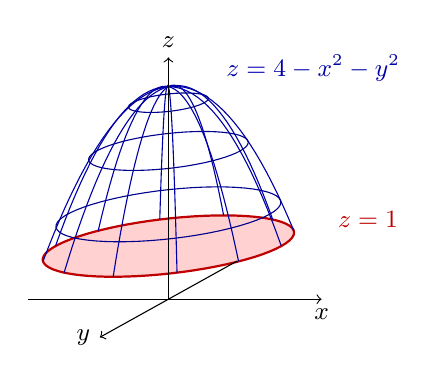
\begin{tikzpicture}[x={(0.92cm,0cm)}, y={(-0.45cm,-0.25cm)}, z={(0cm,0.75cm)}, scale=0.9, every node/.style={font=\small}]
    % Plano z=1 y su circunferencia de intersección con el paraboloide.
    \fill[red!18] plot[domain=0:360, samples=70] ({1.732*cos(\x)},{1.732*sin(\x)},1) -- cycle;
    \draw[red!75!black, thick] plot[domain=0:360, samples=70] ({1.732*cos(\x)},{1.732*sin(\x)},1);

    % Malla del paraboloide z=4-r^2.
    \foreach \angle in {0,30,...,330} {
        \draw[blue!65!black] plot[domain=0:1.732, samples=24]
            ({\x*cos(\angle)},{\x*sin(\angle)},{4-\x*\x});
    }
    \foreach \radius in {0.55,1.10,1.55} {
        \draw[blue!55!black] plot[domain=0:360, samples=60]
            ({\radius*cos(\x)},{\radius*sin(\x)},{4-\radius*\radius});
    }
    \draw[->] (-2.15,0,0) -- (2.35,0,0) node[below] {$x$};
    \draw[->] (0,-2.15,0) -- (0,2.15,0) node[left] {$y$};
    \draw[->] (0,0,0) -- (0,0,4.55) node[above] {$z$};
    \node[blue!65!black] at (2,-0.45,4.2) {$z=4-x^2-y^2$};
    \node[red!75!black] at (2.5,-1.15,1.12) {$z=1$};
\end{tikzpicture}
\end{center}

    \item Evalua: 
\[
\int_0^1\int_0^{\sqrt{x}}\frac{1}{1+y^2}\,dy\,dx.
\]

    \item Evalua: 
\[
\int_0^2\int_{x/2}^{1}e^{y^2}\,dy\,dx.
\]

\end{enumerate}
